% Intended LaTeX compiler: pdflatex
\documentclass[10pt,a4paper,UTF8]{article}
\usepackage{zclorg}
\usepackage{tikztheorem}
\author{张朝龙}
\date{}
\title{练习:内积和范数}
\hypersetup{
 pdfauthor={张朝龙},
 pdftitle={练习:内积和范数},
 pdfkeywords={},
 pdfsubject={},
 pdfcreator={Emacs 25.0.50.1 (Org mode 9.0.6)},
 pdflang={English}}
\begin{document}

\maketitle
\tableofcontents
\titlepic{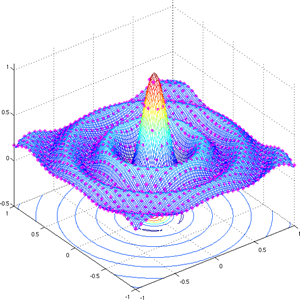
\includegraphics[scale=0.25]{../../img/sinc.PNG}}

\section{6.A.1}
\label{sec:org1e334b2}


\begin{tikzproblem}
证明将\(((x_{1},x_{2}), (y_{1},y_{2}))\in \mathbf{R}^{2}\times \mathbf{R}^{2}\)变为\(|x_{1}y_{1}| + |x_{2}y_{2}|\)的函数不是\(\mathbf{R}^{2}\)上的内积
\end{tikzproblem}

\begin{tikzanswer}
我们需要根据内积的定义来证明。对于内积定义的第三条:第一位置具有可加性。显然有:
\begin{equation}
\label{eq:1}
(((x_{1},x_{2})+(z_{1},z_{2})),(y_{1},y_{2})) = ((x_{1},x_{2}), (y_{1},y_{2})) +((z_{1},z_{2}), (y_{1},y_{2}))
\end{equation}
把\(((x_{1},x_{2}), (y_{1},y_{2}))\in \mathbf{R}^{2}\times \mathbf{R}^{2}\)变为\(|x_{1}y_{1}| + |x_{2}y_{2}|\)。上式的左边是:
\begin{equation}
\label{eq:2}
|x_1y_1 + z_1y_1| + |x_2y_2 + z_2y_2|
\end{equation}
右边是:
\begin{equation}
\label{eq:3}
|x_1y_1| + |x_2y_2| + |z_1y_1| + |z_2y_2|
\end{equation}
左右显然不一定相等,差着一个三角不等式呢。
\end{tikzanswer}
\section{6.A.2}
\label{sec:orgbae0717}


\begin{tikzproblem}
证明将\(((x_{1},x_{2},x_{3}),(y_{1},y_{2},y_{3}))\in \mathbf{R}^{3}\times \mathbf{R}^{3}\)变为\(x_{1}y_{1} + x_{3}y_{3}\)的函数不是\(\mathbf{R}^{3}\)上的内积。
\end{tikzproblem}

\begin{tikzanswer}
这个用内积定义第二条就可以了,我也不知道为什么立即就想到了第二条。
\begin{equation}
\label{eq:4}
((0,1,0),(0,1,0))
\end{equation}
按照题中定义的函数映射结果应该是\(0\),但是,\((0,1,0)\)显然不是\(0\)。违反了第二条。而且,居然跟答案是一样的。
\end{tikzanswer}
\section{6.A.3}
\label{sec:org9c52f03}


\begin{tikzproblem}
设\(\mathbf{F} = \mathbf{R}\)且\(V\neq \{0\}\)。将内积定义中的整形条件改为对某个\(v\in V\)有\(\langle v,v \rangle > 0\)。证明定义中的这个变化并不改变定义了\(V\)上内积的那些从\(V\times V\)到\(\mathbf{R}\)的函数所构成的集合。
\end{tikzproblem}

\begin{tikzanswer}
这个问题我直觉上感觉是可以证明的,但是我又不知道该如何去证明。因为函数的集合里的元素太多了,我不可能一一列举。从特例出发又不可能代表所有。

对某个\(V\)有\(\langle v,v \rangle > 0\), 加上\(V\neq \{0\}\)不妨碍对所有的\(v\in V, \langle v,v \rangle \geq 0\)
\end{tikzanswer}
\section{6.A.4}
\label{sec:org8497da3}


\begin{tikzproblem}
设\(V\)是一个实内积空间。
\begin{enumerate}
\item 证明对所有\(u,v\in V\)均有\(\langle u+v,u-v \rangle   = \| u \|^{2} - \| v \|^{2}\)
\item 证明若\(u,v\in V\)具有相同的范数,则\(u+v\)正交与\(u-v\)
\item 利用\(2\)证明菱形的对角线相互垂直。
\end{enumerate}
\end{tikzproblem}

\begin{tikzanswer}
这个题目的证明比较无趣,根据内积定义即可完成。第3步利用前面的结论很容易证明菱形的对角线相互垂直。对于一个平行四边形\(u+v\)和\(u-v\)就是其对角线,如果\(u,v\)范数相同则有\(u+v,u-v\)垂直。从这个角度看菱形还是有点耳目一新的感觉。
\end{tikzanswer}

\section{6.A.5}
\label{sec:orga876859}


\begin{tikzproblem}
设\(V\)是有限维向量空间,并设\(T\in \mathcal{L}(V)\)使得对每个\(v\in V\)均有\(\| Tv \| \leq \| v \|\)证明\(T-\sqrt{2}I\)是可逆的。
\end{tikzproblem}

\begin{tikzanswer}
证明线性映射\(T-\sqrt{2}I\)可逆,我们只需要证明其是单射。假设\(u\in \mathrm{null}(T- \sqrt{2}I)\),则有:
\begin{equation}
\label{eq:5}
(T-\sqrt{2}I)u = 0
\end{equation}
则有\(\| Tu \| = \sqrt{2} \| v \|\),又因为\(\| Tv \| \leq \| v \|\),则\(u=0\)。哦了。
\end{tikzanswer}
\section{6.A.6}
\label{sec:orgbba7a71}


\begin{tikzproblem}
设\(u,v\in V\) 证明\(\langle u,v \rangle = 0\) 当且仅当对所有\(a\in \mathbf{F}\) 均有 \(\| u \| \leq \| u + av \|\)
\end{tikzproblem}

\begin{tikzanswer}
首先证明当对所有\(a\in \mathbf{F}\) 均有 \(\| u \| \leq \| u + av \|\)时, \(\langle u,v \rangle = 0\)

想到对两边平方然后使用内积定义展开:
\begin{equation}
\label{eq:6}
\langle u,u \rangle  \leq \langle u+av,u+av \rangle
\end{equation}
稍加处理,
\begin{equation}
\label{eq:7}
\langle u,av \rangle + \langle av,u \rangle + |a|^{2} \langle v,v \rangle  \geq 0
\end{equation}
如果上式对所有\(a\)成立。接下来就比较神了。由于对所有的\(a\)成立,所以令:
\begin{equation}
\label{eq:8}
a = - \frac{ \langle u,v \rangle  }{ \| v \|^{2} }
\end{equation}
式 (\ref{eq:7})就变成:
\begin{equation}
\label{eq:9}
-\frac{  | \langle u,v \rangle |^{2}   }{ \| v \|^{2} } \geq 0
\end{equation}
显然必须有\(\langle u,v \rangle   =0\)

另一个方向的证明就不浪费工时了。
\end{tikzanswer}
\section{6.A.7}
\label{sec:org3ef0c68}


\begin{tikzproblem}
设\(u,v\in V\),证明\(\| au + bv \| = \| av + bu \|\)对所有\(a,b\in \mathbf{R}\)均成立,当且仅当\(\| u \| = \| v \|\)
\end{tikzproblem}

\begin{tikzanswer}
首先证明当\(\| u \| = \| v \|\)时,\(\| au + bv \| = \| av + bu \|\)对所有\(a,b\in \mathbf{R}\)均成立。

\begin{eqnarray}
\label{eq:10}
\| au + bv \|^{2} &=& \langle au + bv, au + bv \rangle  \\
&=& |a|^{2} \langle u,u \rangle  + a\bar{b} \langle u,v \rangle + b\bar{a} \langle v,u \rangle  + |b|^{2} \langle v,v \rangle
\end{eqnarray}
\begin{eqnarray}
\label{eq:11}
\| av + bu \|^{2} &=& \langle av+bu,av+bu \rangle  \\
&=& |a|^{2} \langle v,v \rangle + a\bar{b} \langle v,u \rangle + b\bar{a} \langle u,v \rangle + |b|^{2} \langle u,u \rangle
\end{eqnarray}

如果\(\| u \| = \| v \|\),则对比\textasciitilde{}(\ref{eq:10})(\ref{eq:11})有,等式成立。(这里我默认了当\(\| u \|  = \| v \|\)时,有\(\langle u,v \rangle  = \langle v,u \rangle\) )。这个结论可以从 \(\langle u,v \rangle   =  \| u \| \| v \|\cos(\theta)\)得出。其中\(\theta\)是\(u,v\)的夹角。
\end{tikzanswer}
\section{6.A.10}
\label{sec:orgd129035}


\begin{tikzproblem}
求向量\(u,v\in \mathbf{R}^{2}\)使得\(u\)是\((1,3)\)的标量倍,\(v\)正交与\((1,3)\)且\((1,2) = u+ v\)
\end{tikzproblem}

\begin{tikzanswer}
关键词:投影算子。我们要找到\((1,2)\)在\((1,3)\)上的投影,然后\((1,2)\)减去这个投影就是垂直于\((1,3)\)的向量了。

\((1,2)\)在\((1,3)\)上的投影是\((1,3)\)的标量倍。领这个标量是\(c\):
\begin{equation}
\label{eq:12}
c = \frac{ \langle (1,2),(1,3) \rangle  }{ \langle (1,3),(1,3) \rangle  }
\end{equation}
得\(c = \tfrac{7}{10}\),然后一切就很简单了:
\begin{equation}
\label{eq:13}
(1,2) = \frac{7}{10}(1,3) + ( (1,2) - \frac{7}{10}(1,3) )
\end{equation}
\end{tikzanswer}
\section{6.A.11}
\label{sec:org1c016d2}


\begin{tikzproblem}
证明对所有正整数\(a,b,c,d\),均有\(16 \leq (a+b+c+d)(\tfrac{1}{a} + \tfrac{1}{b} + \tfrac{1}{c} + \tfrac{1}{d})\)
\end{tikzproblem}

\begin{tikzanswer}
柯西施瓦茨不等式:设\(u,v\in V\),则 \(| \langle u,v \rangle  | \leq \| u \| \| v \|\)。

对于本题,我们只需要令:
\begin{eqnarray}
\label{eq:14}
u&=& (\sqrt{a},\sqrt{b},\sqrt{c},\sqrt{d}) \\
v&=& (1/\sqrt{a},1/\sqrt{b},1/\sqrt{c},1/\sqrt{d})
\end{eqnarray}
则我们有:
\(| \langle u,v \rangle  |^{2} \leq \| u \|^{2} \| v \|^{2}\)。
原命题得证。
\end{tikzanswer}
\section{6.A.12}
\label{sec:orga9c4d74}


\begin{tikzproblem}
证明对所有正整数\(n\)和实数\(x_{1},\ldots ,x_{n}\),均有\((x_{1} + \ldots + x_{n})^{2} \leq n (x_{1}^{2} + \ldots + x_{n}^{2})\)
\end{tikzproblem}

\begin{tikzanswer}[柯西施瓦茨定理]
因为对于\(\mathbf{x} = (x_{1},\ldots ,x_{n}), \mathbf{y} = (1,\ldots ,1)\),我们有:
\begin{equation}
\label{eq:15}
| \langle x,y \rangle  | \leq \| x \| \| y \|
\end{equation}
有:
\begin{equation}
\label{eq:16}
| \langle x,y \rangle  |^2 \leq \| x \|^2 \| y \|^2
\end{equation}
\end{tikzanswer}
\section{6.A.13}
\label{sec:orge33f92a}


\begin{tikzproblem}
设\(u,v\)是\(\mathbf{R}^{2}\)中的非零向量,证明\(\langle u,v \rangle  = \| u \| \| v \|\cos(\theta)\),其中\(\theta\)是\(u\)和\(v\)的夹角
\end{tikzproblem}

\begin{tikzanswer}
此处需要想象力:一个三角形,有两条边分别是\(u,v\),夹角是\(\theta\),这个角的对边是\(u-v\),有余弦定理:
\begin{equation}
\label{eq:17}
\| u-v \|^{2} = \| u \|^{2} + \| v \|^{2} - 2 \| u \| \| v \|\cos(\theta)
\end{equation}
带入范数定义。得证。

这道题目的关键是\href{https://zh.wikipedia.org/wiki/\%25E9\%25A4\%2598\%25E5\%25BC\%25A6\%25E5\%25AE\%259A\%25E7\%2590\%2586}{余弦定理}。
\end{tikzanswer}
\section{6.A.14}
\label{sec:org0de39c7}


\begin{tikzproblem}
\(\mathbf{R}^{2}\)和\(\mathbf{R}^{3}\)中两个向量的夹角可以用几何的方法来定义。但是对\(n > 3\),\(\mathbf{R}^{n}\)中的几何是难以想象的。所以两个非零向量\(x,y\in \mathbf{R}^{n}\)的夹角定义为\(\arccos \tfrac{\langle x,y \rangle  }{ \| x \| \| y \| }\)。这个定义的动机来源于上一个题目。解释一下为什么这个定义是有意义的。
\end{tikzproblem}

\begin{tikzanswer}
柯西施瓦茨不等式。 \(| \langle u,v \rangle  |  \leq \| u \| \| v \|\) 。两个向量的内积小于等于各自范数的乘积。所以 \(\tfrac{\langle x,y \rangle  }{ \| x \| \| y \| }\)的取值范围是\([-1,1]\),正好符合\(\cos\)函数的取值范围。
\end{tikzanswer}
\section{6.A.15}
\label{sec:org83aa824}


\begin{tikzproblem}
证明对所有实数\(a_{1},\ldots ,a_{n}\)和\(b_{1},\ldots ,b_{n}\)均有:
\begin{equation}
\label{eq:18}
\bigg( \sum_{j=1}^{n} a_{j}b_{j} \bigg)^{2} \leq \bigg( \sum_{j=1}^{n} ja_{j}^{2} \bigg) \bigg( \sum_{j=1}^{n} \frac{b_{j}^{2}}{j} \bigg)
\end{equation}
\end{tikzproblem}

\begin{tikzanswer}
令\(u = (\sqrt{1}a_{1}, \sqrt{2}a_{2},\ldots ,\sqrt{j}a_{j},\ldots ,\sqrt{n}a_{n})\),\(v = \frac{b_{1}}{\sqrt{1}} , \frac{b_{2}}{\sqrt{2}},\ldots , \frac{b_{j}}{\sqrt{j}},\ldots ,\frac{b_{n}}{\sqrt{n}}\)。

剩下来的就交给柯西施瓦茨多项式好了。\(| \langle u,v \rangle  | \leq \| u \| \| v \|\) 。
\end{tikzanswer}
\section{6.A.16}
\label{sec:orge6d3ec5}


\begin{tikzproblem}
设\(u,v\in V\),使得\(\| v \|=3, \| u-v \| = 6, \| u+v \| = 4\), \(\| u \|\)等于多少?
\end{tikzproblem}

\begin{tikzanswer}
这个是那个有名的平行四边形定理:平行四边形四条边的模的和等于对角线的模的和。显然有 \(\| u \| = \sqrt{17}\)

\begin{equation}
\label{eq:19}
 \| u-v \|^{2} + \| u+v \|^{2} = 2( \| u \|^{2} + \| v \|^{2} )
\end{equation}
\end{tikzanswer}
\section{6.A.17}
\label{sec:org6fd80fc}


\begin{tikzproblem}
证明或反驳: \(\mathbf{R}^{2}\)上有一个内积使得该内积确定的范数为:对所有的\((x,y)\in \mathbf{R}^{2}\)有: \(\| (x,y) \| = \max\{|x|,|y|\}\)
\end{tikzproblem}

\begin{tikzanswer}
任何一个满足题中条件的内积好像不满足内基定义的第一个位置的加性。这么快就被我识破了。
\end{tikzanswer}
\section{6.A.18}
\label{sec:org2f0761b}


\begin{tikzproblem}
设\(p > 0\),证明\(\mathbf{R}^{2}\)上有一个内积使得该内积确定的范数为:
\begin{equation}
\label{eq:20}
\forall (x,y)\in \mathbf{R}^{2}\quad \| (x,y) \| = ( |x|^{p} + |y|^{p} )^{1/p}
\end{equation}
当且仅当\(p=2\)
\end{tikzproblem}

\begin{tikzanswer}
首先当\(p=2\)时,点积和欧几里得范数满足给定结论。我们需要证明\(p\neq 2\)时,不存在这个内积。

假设\(p\neq 2\)且存在内积满足给定的范数:
\begin{equation}
\label{eq:21}
\| (1,0) + (0,1) \|^{2} + \| (1,0) - (0,1) \|^{2} = 2 ( \| (1,0) \|^{2} + \| (0,1) \|^{2} )
\end{equation}
上式变成:
\begin{equation}
\label{eq:22}
2^{2/p} + 2^{2/p} = 2 (1^{2} + 1^{2})
\end{equation}
有\(2^{2/p} = 2\),这与\(p\neq 2\)矛盾。
\end{tikzanswer}
\section{6.A.19}
\label{sec:org1706e55}


\begin{tikzproblem}
设\(V\)是实内积空间,证明对所有的\(u,v\in V\)均有:
\begin{equation}
\label{eq:23}
\langle u,v \rangle  = \frac{ \| u+v \|^{2} - \| u-v \|^{2} }{4}
\end{equation}
\end{tikzproblem}

\begin{tikzanswer}
范数和内积性质结合。得证。
\end{tikzanswer}
\section{6.A.20}
\label{sec:orgc425dbc}


\begin{tikzproblem}
设\(V\)是复内积空间。证明对所有\(u,v\in V\)均有:
\begin{equation}
\label{eq:24}
\langle u,v \rangle = \frac{ \| u+v \|^{2} - \| u-v \|^{2} + \| u+iv \|^{2}i - \| u-iv \|^{2}i }{4}
\end{equation}
\end{tikzproblem}
\begin{tikzanswer}
同上。
\end{tikzanswer}
\section{6.A.21}
\label{sec:org8cbf6f4}


\begin{tikzproblem}
向量空间\(U\)上的范数是满足以下条件的函数\(\|  \|: U \to [0,\infty)\), \(\| u \| = 0\)当且仅当\(u = 0\),对所有的\(\alpha \in \mathbf{F}\)和\(u\in U\),均有\(\| au \| = |a| \| u \|\),对所有\(u,v\in U\)均有\(\| u+v \| \leq \| u \| + \| v \|\)。证明满足平行四边形恒等式的范数均来自于内积。也就是说若\(\|  \|\)是\(U\)上满足平行四边形恒等方式的范数,则有\(U\)上的内积,\(\langle , \rangle\) 使得对所有\(u\in  U\)均有\(\| u \| = \langle u,u \rangle^{1/2}\)
\end{tikzproblem}
\begin{tikzanswer}
按照内积定义,逐条性质证明即可。
\end{tikzanswer}
\section{6.A.22}
\label{sec:org70bfdc3}


\begin{tikzproblem}
证明平均数的平凡小于等于平方的平均数。更确切的说,若\(a_{1},\ldots ,a_{n}\in \mathbf{R}\),则\(a_{1},\ldots ,a_{n}\)的平均数的平方小于等于\(a_{1}^{2},\ldots ,a_{n}^{2}\)的平均数。
\end{tikzproblem}
\begin{tikzanswer}
这道题和6.A.12是一样的。使用柯西施瓦茨不等式。内积的绝对值小于等于范数的乘积。
\end{tikzanswer}
\section{6.A.23}
\label{sec:org445bbcb}


\begin{tikzproblem}
设\(V_{1},\ldots ,V_{m}\)均为内积空间,证明等式:\(\langle\) (u\_1,\ldots ,u\_m),(v\_1,\ldots ,v\_m) \(\rangle\)  = \(\langle\) u\_1,v\_1 \(\rangle\) + \ldots + \(\langle\) u\_m,v\_m \(\rangle\)  定义了\(V_{1}\times \ldots \times V_{m}\)上的内积
\end{tikzproblem}

\begin{tikzanswer}
设\(V_{1},\ldots ,V_{m}\)是\(F\)上的向量空间,则:
\begin{equation}
\label{eq:25}
V_{1}\times \ldots \times V_{m} = \{ (v_{1},\ldots ,v_{m}): v_{1}\in V_{1},\ldots ,v_{m}\in V_{m} \}
\end{equation}
对 \(\langle (u_1,\ldots ,u_m),(v_1,\ldots ,v_m) \rangle  = \langle u_1,v_1 \rangle + \ldots + \langle u_m,v_m \rangle\)   定义了\(V_{1}\times \ldots \times V_{m}\)按照内积定义的性质逐条证明即可。

\(V\)上的内积就是一个函数,把\(V\)中的元素的每个有序对\(u,v\)都映成一个数\(\langle u,v \rangle\) 并且具有以下性质:
\begin{enumerate}
\item 对所有的\(v\in V\),有\(\langle v,v \rangle \geq 0\)
\item \(\langle v,v \rangle =  0\),当且仅当\(v=0\)
\item 对所有\(u,v,w\in V\),均有\(\langle u+v,w \rangle = \langle u,w \rangle + \langle v,w \rangle\)
\item 对所有\(\lambda\in \mathbf{F}\)和所有\(u,v\in V\),有\(\langle \lambda u,v \rangle = \lambda \langle u,v \rangle\)
\item 对所有\(u,v\in V\),有\(\langle u,v \rangle = \overline{ \langle v,u \rangle }\)
\end{enumerate}
\end{tikzanswer}
\end{document}
